\chapter{Processing Pipeline}
\label{ch:processing_pipeline}

\cref{ch:dataset,ch:argus} discuss methods to curate and augment datasets. Using these datasets, we train a \gls{nn} to develop a processing pipeline. This chapter describes this process and how we developed our pipeline to detect bib sheets `in-the-wild' on any given marathon photo. Lastly, we explain our method of \gls{ocr} to convert our \gls{rbn} candidates into text.  An overview of our pipeline is shown in \cref{fig:processing_pipeline:pipeline} and the source code is made available online\footnoteurl{http://github.com/alexcu/hermes-bib-detect}{25 September 2017}.

\begin{figure}[h]
  \centering
  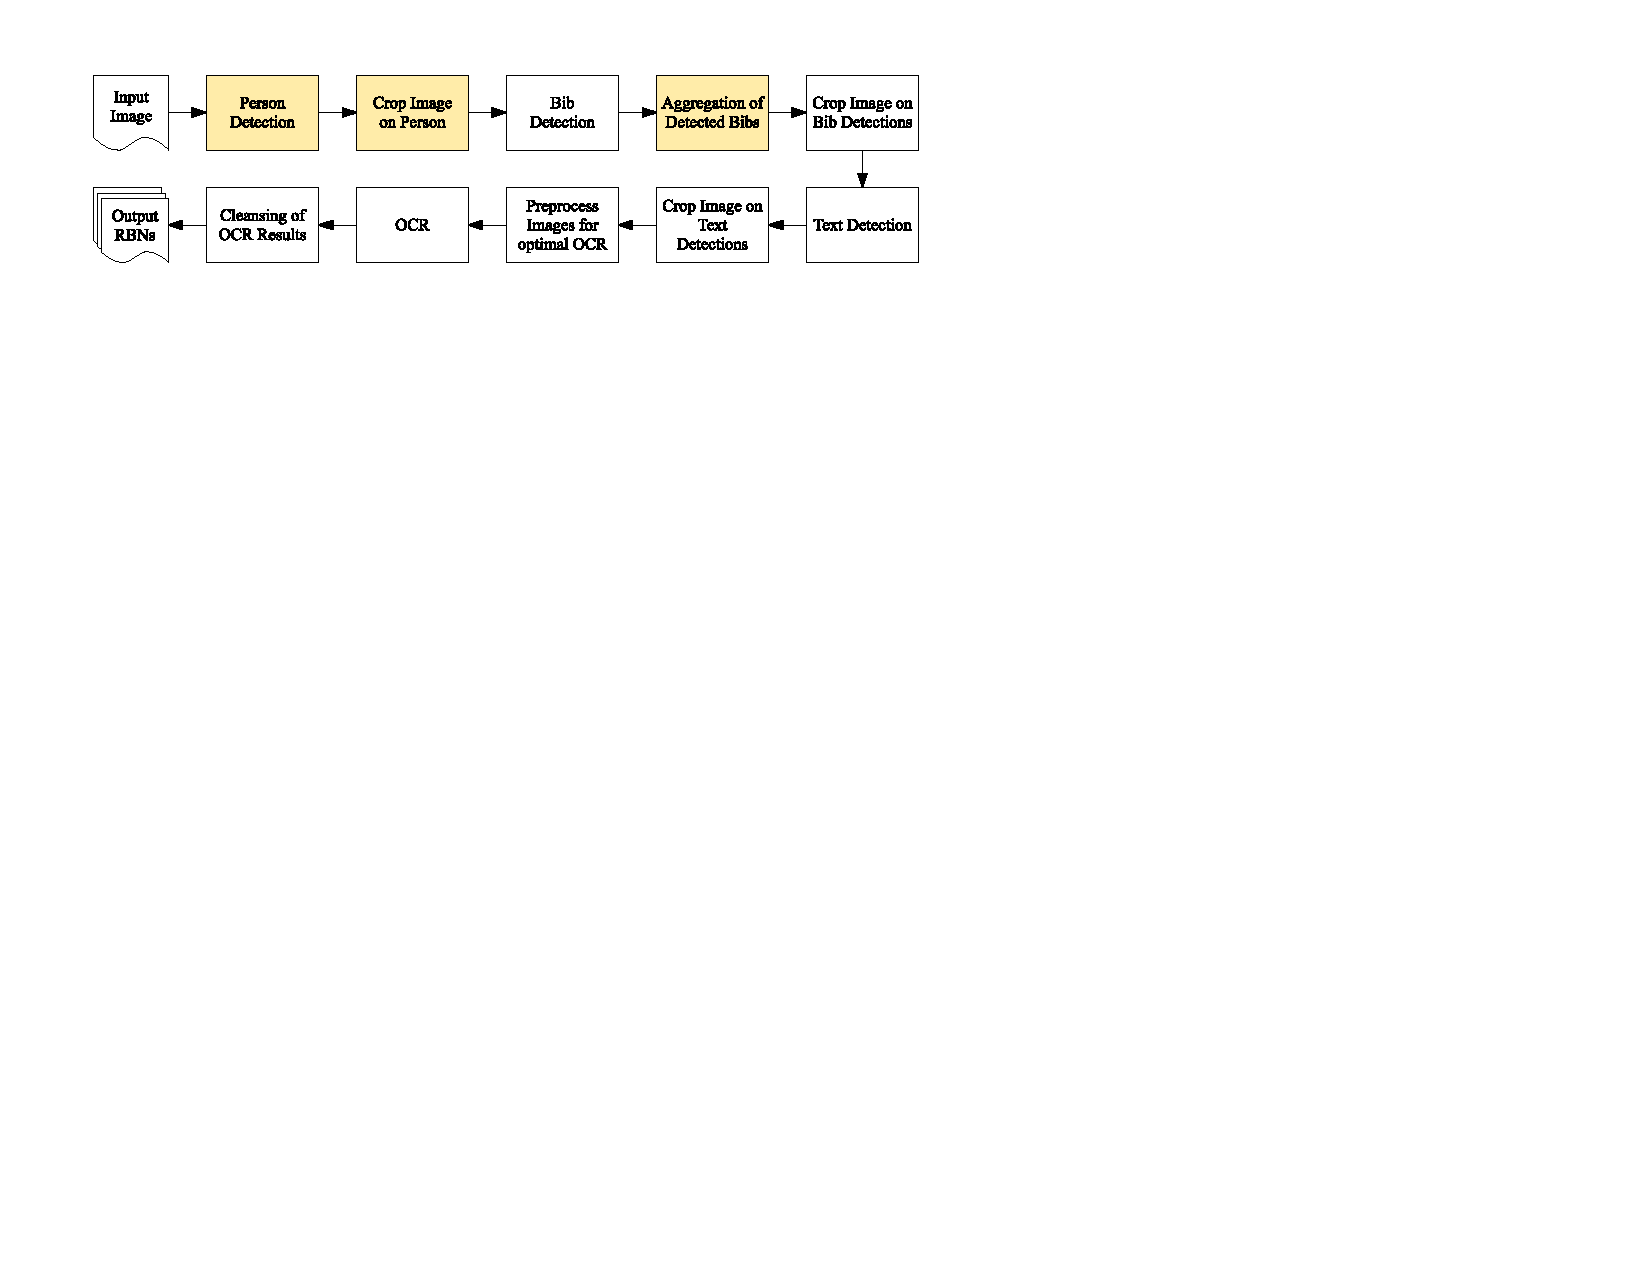
\includegraphics[width=\textwidth]{images/processing/pipeline}
  \caption[Overview of our processing pipeline]{A high level overview of our processing pipeline. Highlighted components indicate optional steps that, when included, are proposed to increase accuracy. We use the stereotypes \texttt{$<<$NN$>>$} and \texttt{$<<$Heuristic$>>$} to differentiate between \gls{nn}-based and heuristic-based components.}
  \label{fig:processing_pipeline:pipeline}
\end{figure}

\section{Bib Detection}
\label{sec:processing_pipeline:pipeline}

Detecting bibs in an image is a image segmentation problem. There are multiple approaches that address this issue: typical approaches from literature in the area have used heuristic-based methods to segment an image, as highlighted in \cref{sec:background:detection_strategies}. As this research is part of a wider project under \gls{dstil}, three heuristic-based approaches were investigated in addition to the  \gls{ai} approach proposed by this study. 

\subsection{Existing Approaches}
\label{sec:processing_pipeline:bib_detection:existing_approaches}

The first was face detection and heuristics to find the bib--as presented in \citep{Benami:2012jf}---though as shown in \cref{fig:background:recognition:benami2012_missed}, this approach does not always work. To combat the issue of subjects leaning in photos, we looked at a two further heuristic-supported approaches: poselet detection to detect a human skeleton \citep{Nguyen:2015vc} and using a pre-trained \gls{cnn} running the \gls{yolo} object-detection system \citep{redmon2016yolo9000} on the Darknet framework \citep{darknet13}. We discuss the person detection in more detail within \cref{sec:processing_pipeline:person_filtering}. In the latter, we only attempted to look at object detection of people. Both methods produced greater person detection candidate areas than using face areas alone, and we processed  these results we used similar visual processing to that of \citet{Benami:2012jf}, albeit on a larger detection area.

But---as per the aims of this research---can a detection strategy be achieved without using heuristic-based approaches at all? We discuss our solution for solving this question using deep-learning \glspl{nn} in the following section.

\subsection{Deep-Learning Approaches}
\label{sec:processing_pipeline:bib_detection:deep_learning}

\def \frcnn {Faster \gls{rcnn}}

\cref{sec:background:detection:learning} introduced applications of deep-learning, specifically \glsplx{cnn}, that were successfully applied on object instance segmentation within images. We investigate similar approaches for recognising racer's bib sheets using the data collected from Argus  (\cref{ch:argus}).

To implement our approach, we explored the viability of using region-based \glspl{cnn}, known as \glspl{rcnn}. These were first introduced by \citet{Girshick:2014jx} in \citeyear{Girshick:2014jx}, and more than doubled the accuracy of previous object detection methods such as \gls{hog} \citep{Dalal:2005jq} and \gls{sift} \citep{Lowe:2004kp}. The \gls{rcnn} approach was improved upon with \textit{Fast \gls{rcnn}} \citep{Girshick:2015vr} that increased detection speed. We adopted the \gls{rcnn} approach that was improved upon in a  recent \citeyear{Ren:2017ug} study, \textit{\frcnn{}} \citep{Ren:2017ug}, to predict bib regions. \frcnn{} combines \glspl{cnn} with state-of-the-art object detection networks (e.g., region proposal algorithms). The sharing of convolutional layers of a \gls{cnn} with object detection networks produces an \gls{rpn} that is utilised by \frcnn{}.

We applied \frcnn{} to the context of bib detection by the process of transfer learning \cite{Caruana:1997wk,Thrun:1996wh,Baxter:1997wr}: this involves adjusting the final layer of a pre-trained \gls{nn} and adding a context-specific layer (in our case, racing bibs). The concept of transfer learning mimics that of human learning in that humans do not learn tasks in isolation, but a sequence of training tasks over a lifetime. (If one has learnt English and Latin, then learning French is easier due to transfer learning.) Transfer learning has successfully been applied to various contexts such as spam filtering \citep{Bickel:2006ul} and text classification \citep{Raina:2006tv, Do:2005uz}.

To implement this detection pipeline, we chose a Keras \citep{chollet2015keras} Python implementation of \frcnn{}\footnoteurl{https://github.com/alexcu/keras-frcnn}{21 August 2017} that runs on top of the TensorFlow \citep{tensorflow2015-whitepaper} library. To reduce false positives, we reject any candidate that is predicted with an accuracy of less than 50\%. However, while we were able to extract a large amount of bibs from many images, there were cases of shoes, signs and hands being detected with accuracies above 90\%. There were also some false negatives due to excessive noise in the photo. \cref{fig:processing_pipeline:bib_only} shows this in further detail. We decided to amend this by cropping each image down to detected people using the \gls{yolo} system.

\begin{figure}[h]
  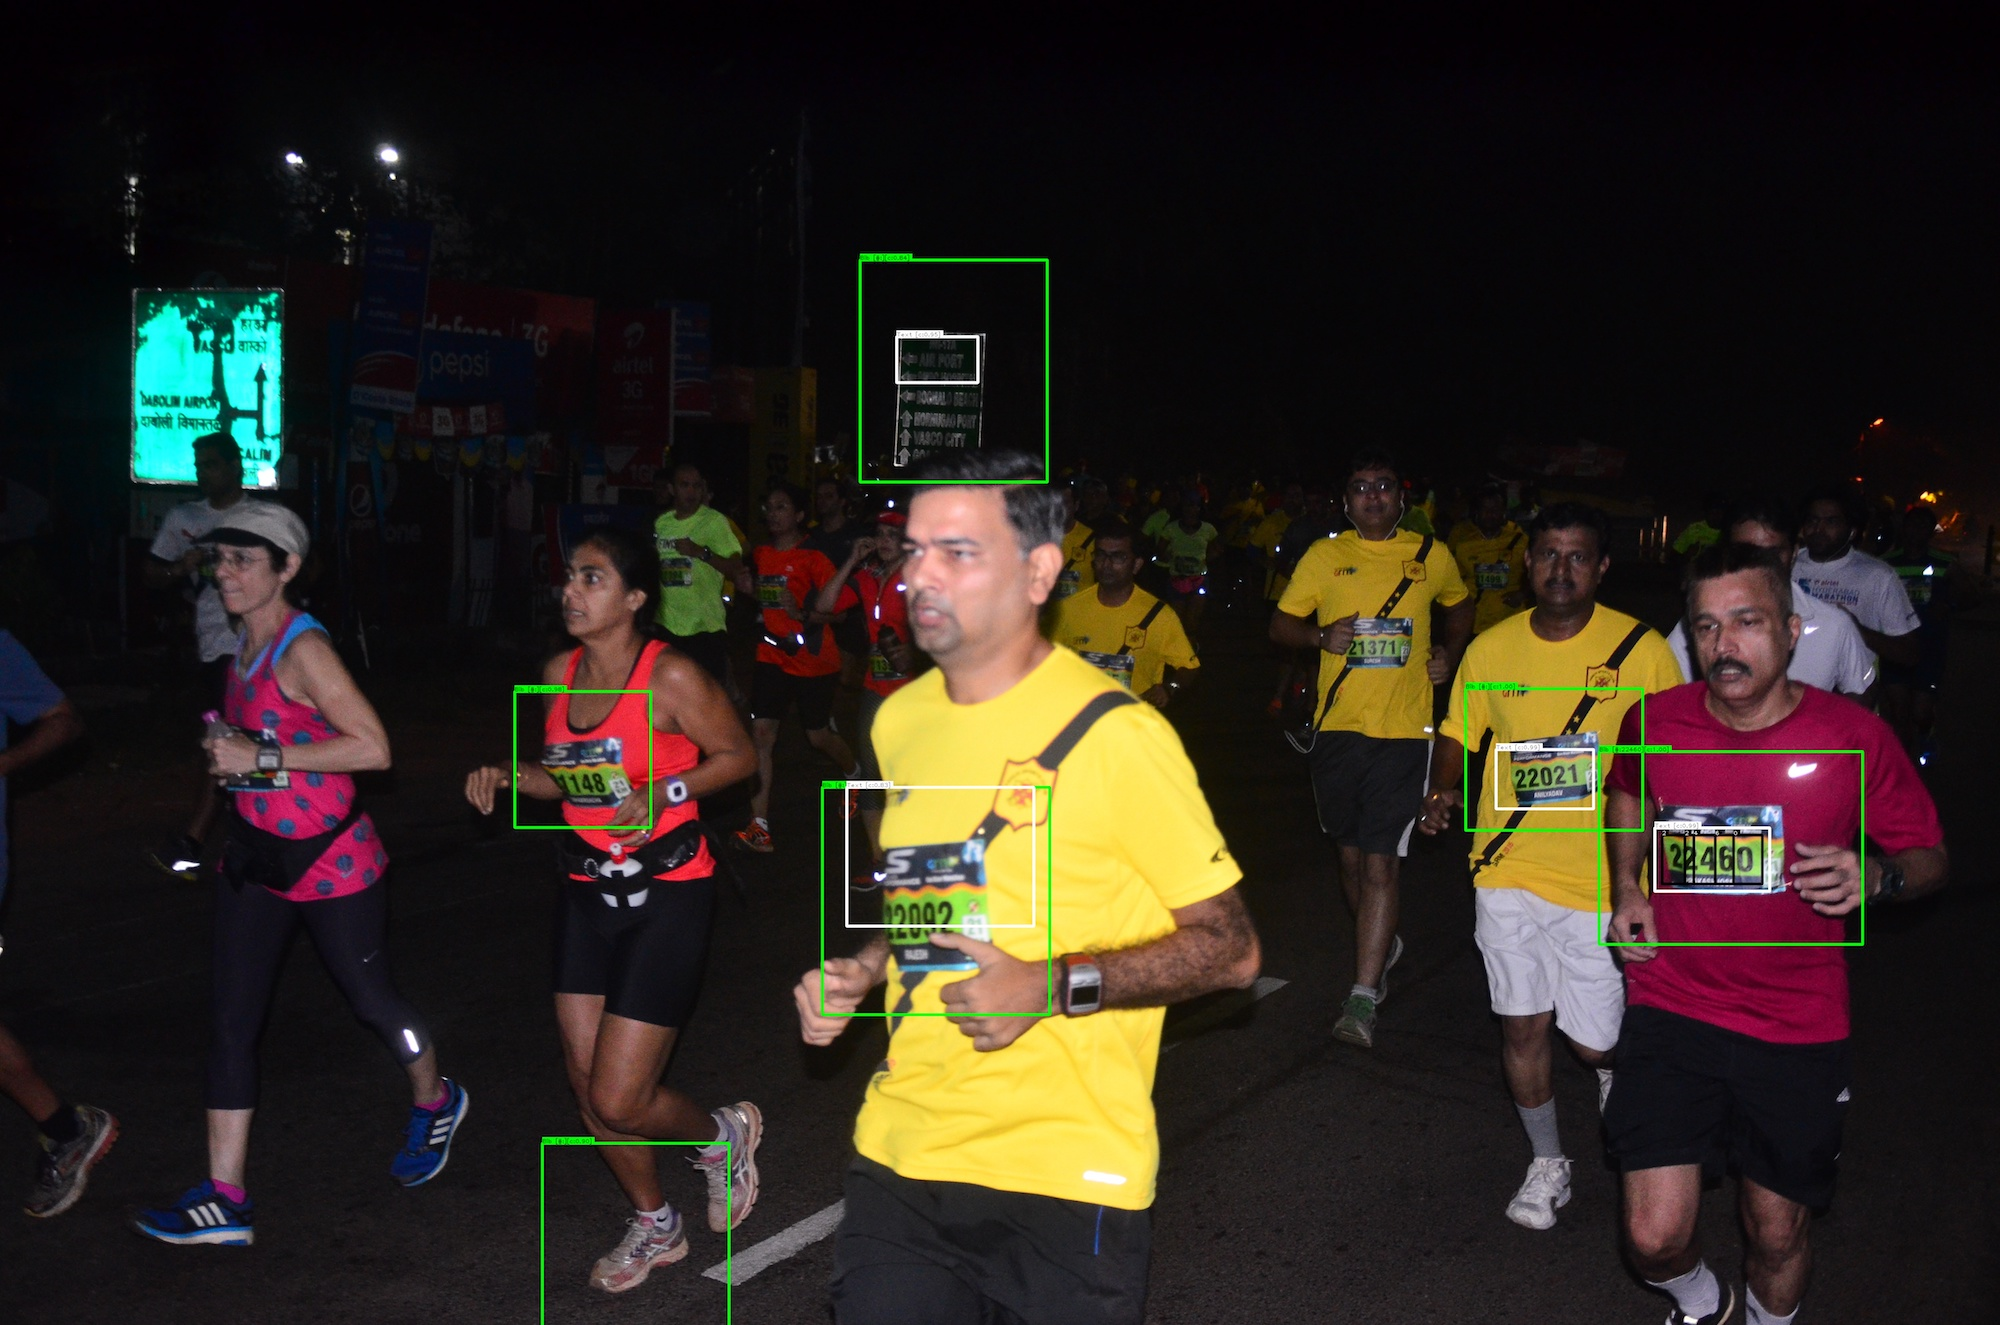
\includegraphics[width=\textwidth]{images/processing/bib_only}
  \caption[Bib detection results using FRCNN]{Results from using \frcnn{} Keras implementation running on TensorFlow. Note the false negative for the third runner from the right and the false positive on the second runner's shoe from the left.}
  \label{fig:processing_pipeline:bib_only}
\end{figure}

% How did we achieve bib detection?
% Technology that we used.
% Keras-FRCNN
% 33,948 bibs over 36,822 images for training and 4,131 images and 4,375 bibs for validation.
% Why FRCNN?
% Why Keras?
% Which implementation?
% Extract all sample images into a CSV.
% Talk about noticeable false negatives in some images.
% How did we fix this? Lead to next section..

\subsection{Person Filtering}
\label{sec:processing_pipeline:person_filtering}

As described in \cref{sec:processing_pipeline:bib_detection:existing_approaches}, a heuristic-based method explored was to apply visual transformation on a person detection to extract the \gls{rbn}. The person detection component used a pre-trained network built on the \gls{yolo} object detection system running on a customised implementation of Darknet\footnoteurl{https://github.com/alexcu/darknet}{21 August 2017}.

We were able to utilise a similar method by extracting people from an image using \gls{yolo} (\cref{fig:processing_pipeline:person_filtering:yolo_crop_person_detection}), and cropping each image to the respective bounding box of the detected areas. Using weights from the Tiny \gls{yolo} model\footnoteurl{https://pjreddie.com/darknet/yolo/\#tiny}{5 September 2017}, \gls{yolo} was able to detect the most prominent runners in the image, with which we found desirable considering the aims of the project. We then ran our \frcnn{} prediction model on each cropped image (\cref{fig:processing_pipeline:person_filtering:yolo_crop_aggregated_detections}). As these images had reduced noise, accuracies of bib detections increased with fewer false positives. 

The last stage of the bib detection was to aggregate all detections of separate runners back into one image (\cref{fig:processing_pipeline:person_filtering:yolo_crop_aggregated_detections}), and union overlapping predicted regions (\cref{fig:processing_pipeline:person_filtering:yolo_crop_unioned_detections}). (We found that in some cases, two or more bibs would be detected in a single person crop due to runner's in the background.) In some cases, however, it was unwise to union \textit{all} overlapping regions, such as that shown in \cref{fig:processing_pipeline:hand}. Using $a(r)$ to denote the area of a region, we only formed the union of both regions, $r_{1} \cup r_{2}$, if the area of the intersection region, $a(r_{1} \cap r_{2})$, was more than 75\% of the area of one of the area of one of the regions.

\begin{figure}[h]
  \centering
  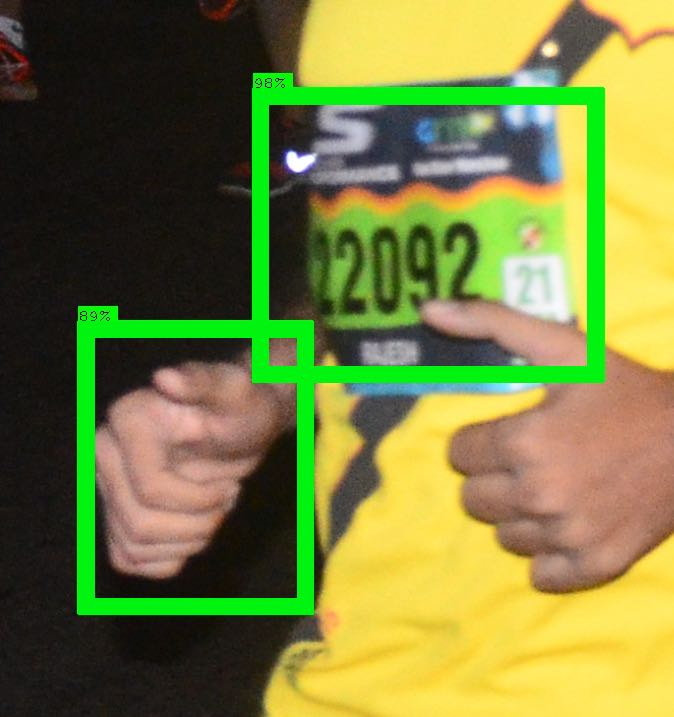
\includegraphics[width=0.3\textwidth]{images/processing/hand}
  \caption[Invalid intersection to union both regions]{Invalid intersection to union both regions. The area of the intersection is not greater than 75\% of the two regions.}
  \label{fig:processing_pipeline:hand}
\end{figure}

Thus, given $N$ detected runners in a single image with $N$ cropped images, let $R$ represent the union\footnote{Here, \textit{union} refers to a union in set theory.} of all regions $r$ for the $n$th crop to produce \cref{fig:processing_pipeline:person_filtering:yolo_crop_aggregated_detections}. The final regions, $R_{f}$, of an image are all regions, $R$, and union regions, $R_{u}$ but not intersection regions, $R_{i}$. Therefore, the process of overlapping (\cref{fig:processing_pipeline:person_filtering:yolo_crop_unioned_detections}) can formally be described in set notation:
\begin{align*}
% A(r1, r2) is a function that accepts both r1 and r2 and returns true if a(r1 or r2) > 0.75 a(intersection(r1, r2)) 
A(r_{1}, r_{2}) &= (\ a(r_{1} \cap r_{2}) > 0.75 \times a(r_{1})\ ) \ \vee \ (\ a(r_{1} \cap r_{2}) > 0.75 \times a(r_{2})\ )\\
% Ru is the union of all intersections that match A(..)
R_{u} &= \{\ r_{1} \cup r_{2}\ |\ (r_{1}, r_{2}) \in R \ \wedge\ r_{1} \neq r_{2} \ \wedge\  A(r_{1}, r_{2})\ \}\\
% Ri is there exists a single r in R and for all other rx's in R, r ≠ rx and A(..), we return that r as rx will be swapped in the forall
R_{i} &= \{\ r \ |\ (\exists r \in R)(\forall r_{x} \in R)[\ r \neq r_{x}\ \wedge\  A(r, r_{x})\ ]\ \}\\
R_{f} &= \{\ r\ |\ r \in R \wedge r \in R_{u} \wedge r \not\in R_{i}\ \}
\end{align*}

These overlaps increased the likelihood of extracting the \gls{rbn} given a larger extraction image.

\begin{landscape}
  \begin{figure}[p]
    \centering
    \begin{subfigure}[b]{0.23\paperwidth}
      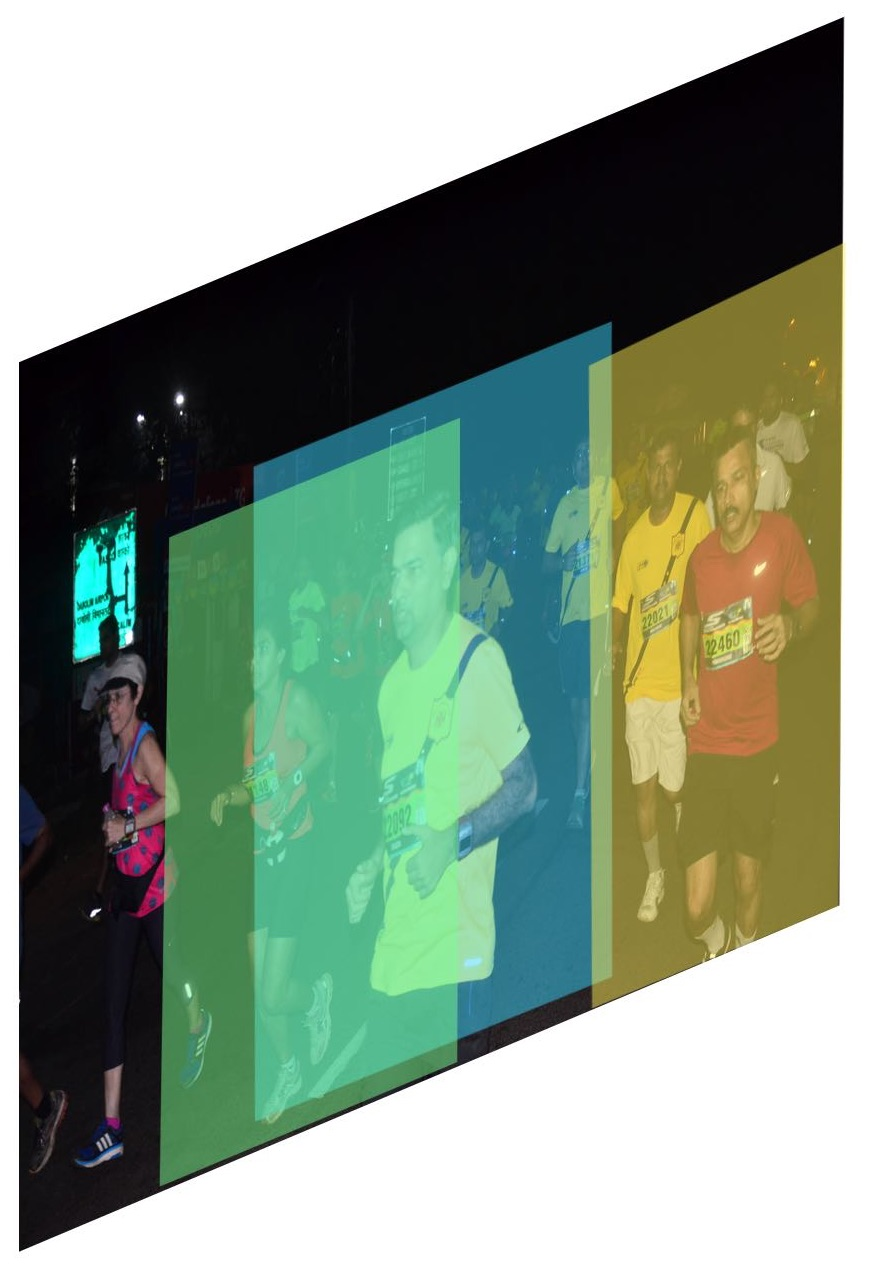
\includegraphics[width=\textwidth]{images/processing/yolo_crop_person_detection}
      \caption{Person detection}
    \label{fig:processing_pipeline:person_filtering:yolo_crop_person_detection}
    \end{subfigure}
    \begin{subfigure}[b]{0.23\paperwidth}
      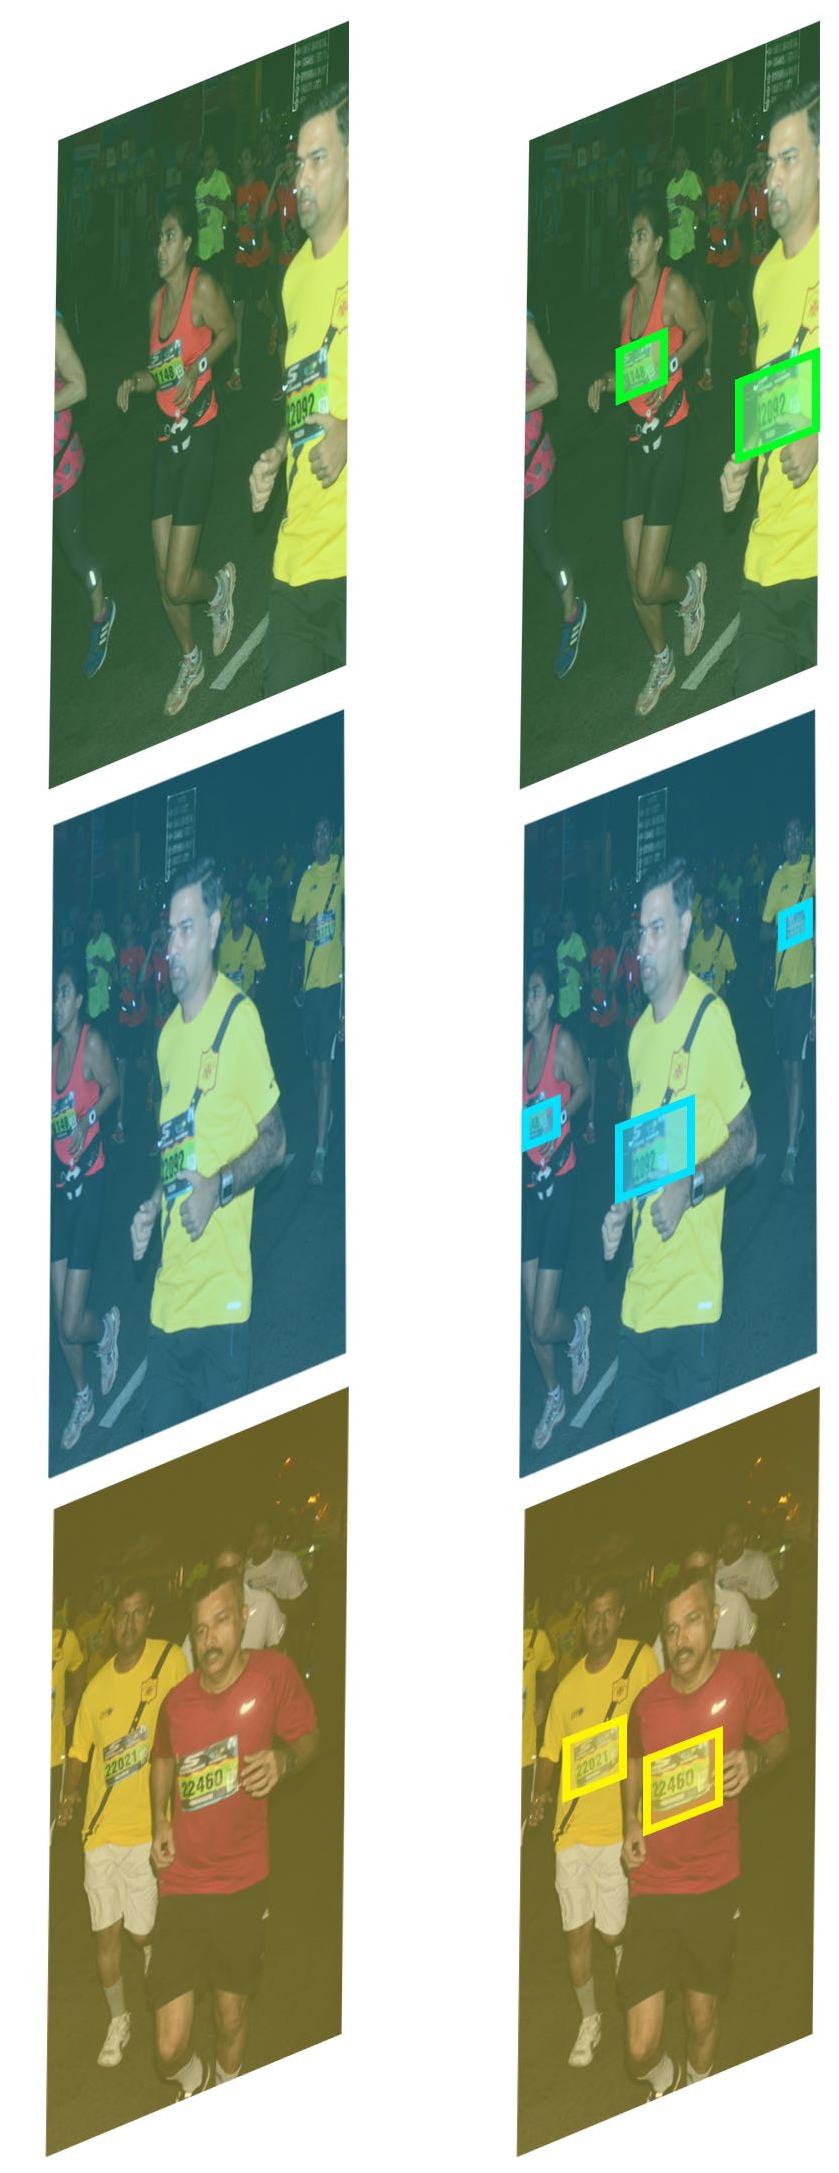
\includegraphics[width=\textwidth]{images/processing/yolo_crop_bib_detection}
      \caption{Bib detection}
      \label{fig:processing_pipeline:person_filtering:yolo_crop_bib_detection}
    \end{subfigure}
    \begin{subfigure}[b]{0.23\paperwidth}
      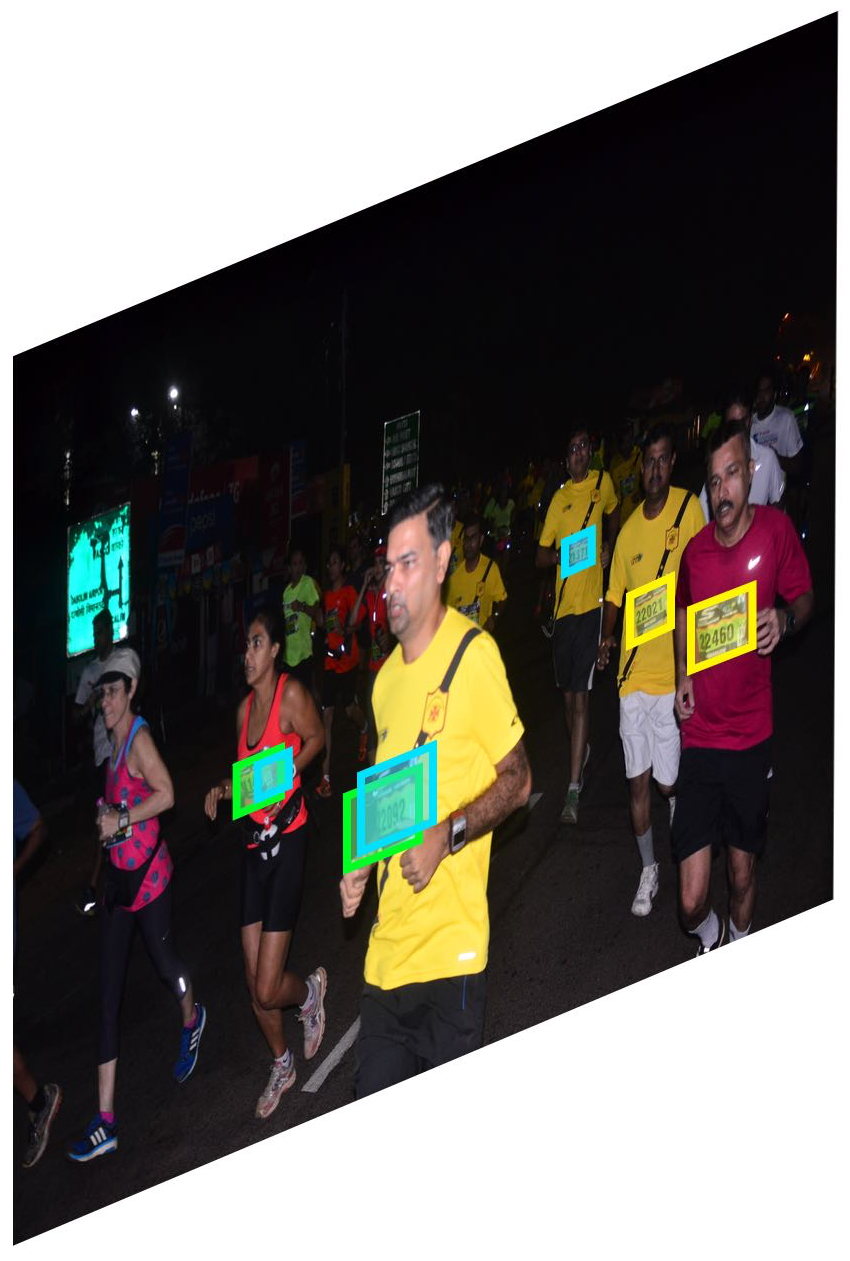
\includegraphics[width=\textwidth]{images/processing/yolo_crop_aggregated_detections}
      \caption{Aggregation}
      \label{fig:processing_pipeline:person_filtering:yolo_crop_aggregated_detections}
    \end{subfigure}
    \begin{subfigure}[b]{0.23\paperwidth}
      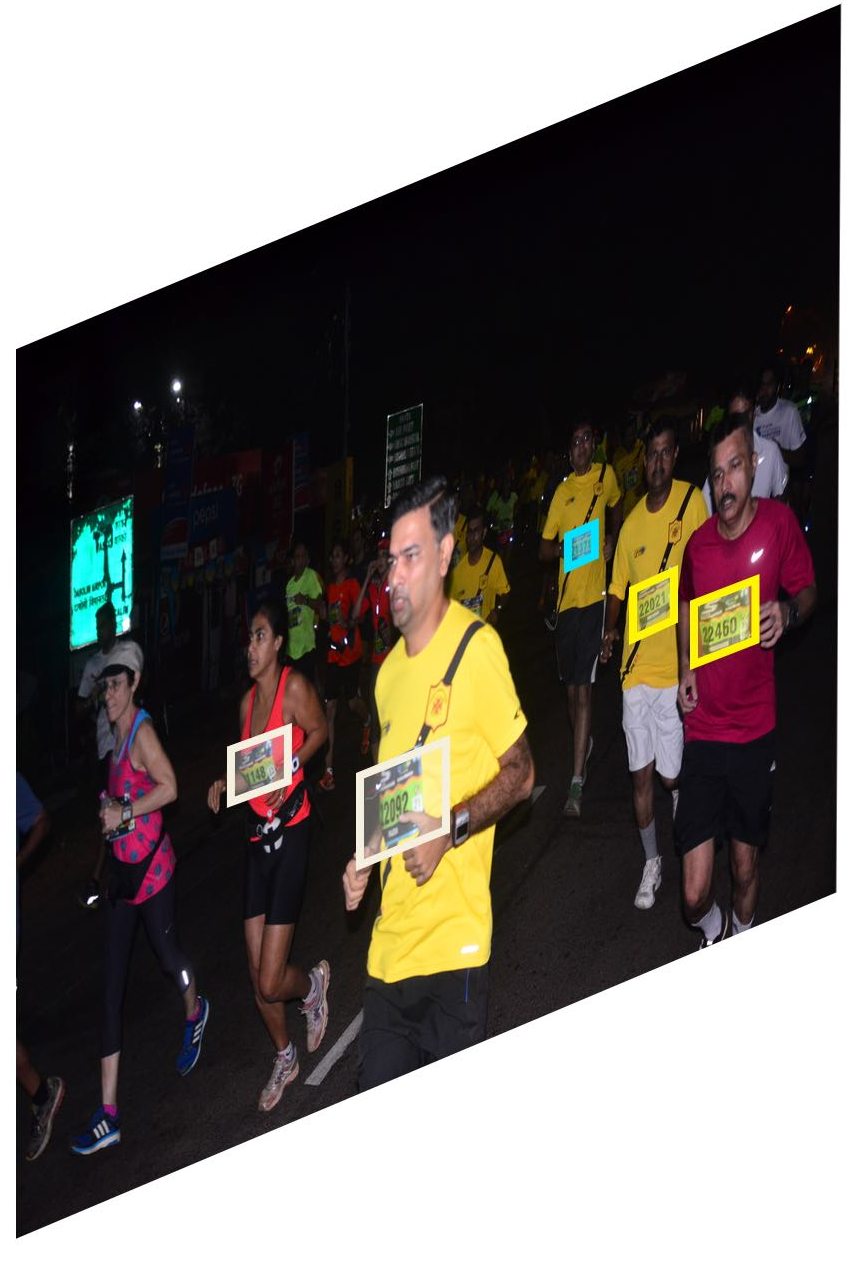
\includegraphics[width=\textwidth]{images/processing/yolo_crop_unioned_detections}
      \caption{Overlapping}
      \label{fig:processing_pipeline:person_filtering:yolo_crop_unioned_detections}
    \end{subfigure}
    \caption[Person filter using YOLO to improve accuracies of bib detection]{Improving accuracies of bib detection by cropping people. (a): Three bounding boxes detected for \textsc{people} using \gls{yolo}. (b): Bib detections from \frcnn{} (right) on each person crop (left). (c): Aggregated bib detections from individual person crops. Note the two overlapping blue and green regions. (d): The union of overlapped regions are merged into a single region, shown in white.}
    \label{fig:processing_pipeline:person_filtering}
  \end{figure}
\end{landscape}

% To improve the false negative rates, we crop the images down to individual detected persons.
% How?
% Use person detection from YOLO + Darknet
% Train YOLO to detect people
% From people detections we only
% YOLO was good at getting more prominent runners, which is what we wanted


% Run the bib detection on each of the cropped individual images.
% From this, union each of the bibs detected (overlaps).
% Why? Greater area of circumference
% Reduce false positives by heuristic if width < height then reject
\section{Text Detection}

The penultimate stage of the pipeline is to crop each bib detection region and focus on the \gls{rbn} itself, as shown in \cref{fig:processing_pipeline:text_detection}. We attempted to train \frcnn{} using both the \gls{coco}-Text \citep{Veit:2016vj} and SynthText In The Wild \citep{Gupta:2016ws} datasets, following a similar process outlined in \cref{sec:processing_pipeline:bib_detection:deep_learning}. However, we found that---due to the wide variance of typeface samples within the \gls{coco}-Text dataset---\frcnn{} was only able to make reliable predictions on the SynthText dataset. Thus, we determined that \frcnn{} is suitable for text extraction given that it is trained on a dataset where text samples similar (i.e., the consistency of the synthetic words generated in the SynthText dataset made this possible).

Text detection used for two key purposes. Firstly, this helps to reduce false positives in the bib detection stage as if no text regions could be found, we assume the candidate region is not a bib image. Secondly, we use the largest text region on the bib found to pass feed into a text recognition engine. We explain this in the following section.

\begin{figure}[h]
  \centering
  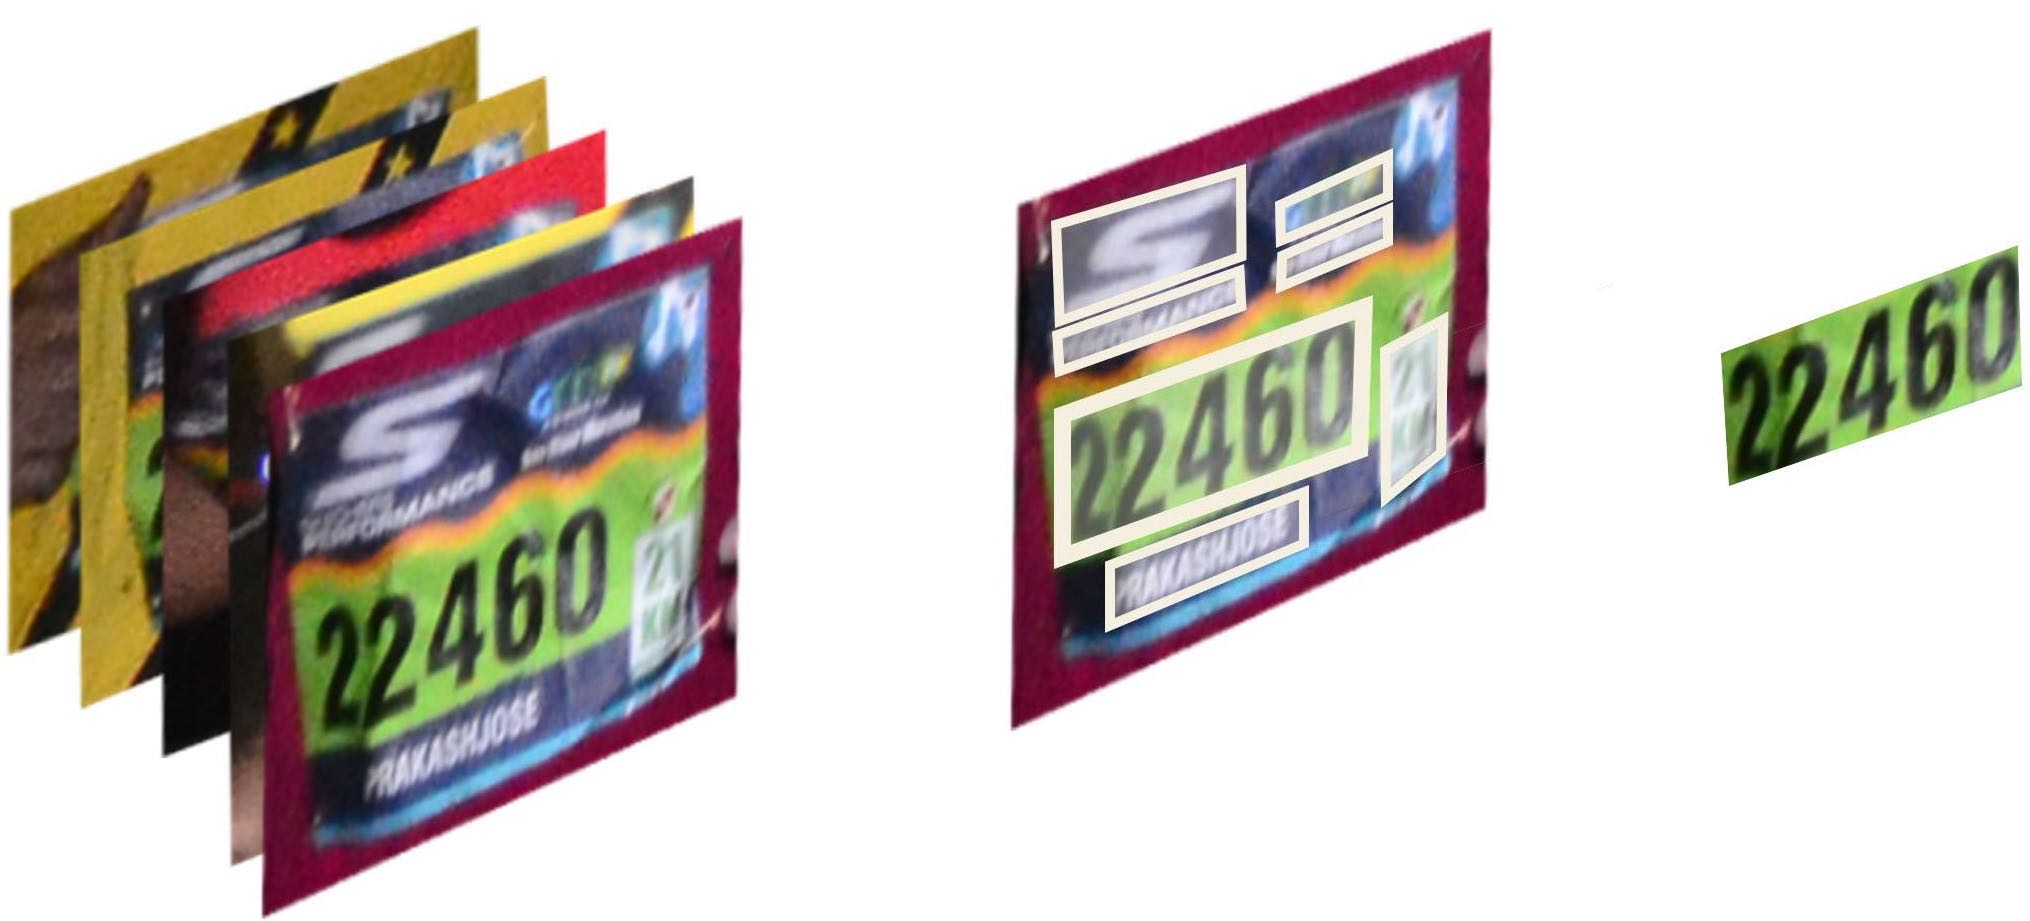
\includegraphics[width=\textwidth]{images/processing/text_process}
  \caption[Text region detection pipeline]{Text region detection. Detected bibs are cropped from the original image (left) and parsed through a text detection pipeline (middle). We select the candidate with the largest area and crop it (right).}
  \label{fig:processing_pipeline:text_detection}
\end{figure}

% DID USE THE Scene Text in The Wild....
% Tried to re-use FRCNN, but this network was not good enough. What dataset did we use, tried with COCO-Text but did not work. Tried with SynthText90k?
% Once we find the largest text region on the bib, we can then feed this into tesseract-4 alpha

\section{Text Recognition}

Before we feed the text area into an \gls{ocr} engine, we preprocess the extracted text images to optimise their recognition (\cref{fig:processing_pipeline:ocr_postprocessing}). We produce three preprocessed optimal candidates: greyscale, inverse greyscale, and threshold binary. For images with black and white numbers, we use the statistical median of the image's colour range: where the median is greater than 128, we assume a white number is detected (i.e., white on a darker background, such as \cref{fig:processing_pipeline:ocr_postprocessing:white_on_dark_original}) and apply a binarised inverse threshold on the image. Otherwise, we assume a black number is detected, where we threshold without the inverse. Greyscale and inverse greyscale are most suitable for text regions where \glspl{rbn} are not in a black or white typeface (\cref{fig:processing_pipeline:ocr_postprocessing:color_original}).

\begin{figure}[h]
  \centering
  \begin{subfigure}[b]{0.23\textwidth}
    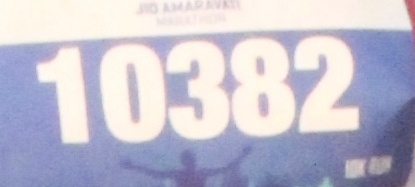
\includegraphics[width=\textwidth]{images/processing/ocr/10382_org}
    \caption{Original Image}
    \label{fig:processing_pipeline:ocr_postprocessing:white_on_dark_original}
  \end{subfigure}
  \hspace{\fill}
  \begin{subfigure}[b]{0.23\textwidth}
    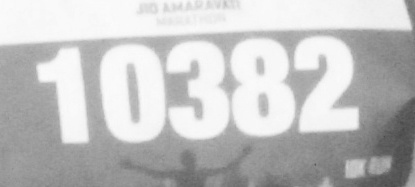
\includegraphics[width=\textwidth]{images/processing/ocr/10382_bw}
    \caption{Greyscale}
  \end{subfigure}
  \hspace{\fill}
  \begin{subfigure}[b]{0.23\textwidth}
    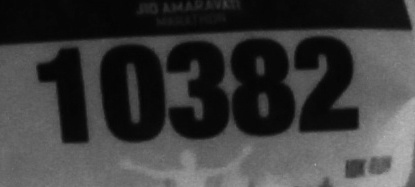
\includegraphics[width=\textwidth]{images/processing/ocr/10382_bw_inv}
    \caption{Inverse Greyscale}
  \end{subfigure}
  \hspace{\fill}
  \begin{subfigure}[b]{0.23\textwidth}
    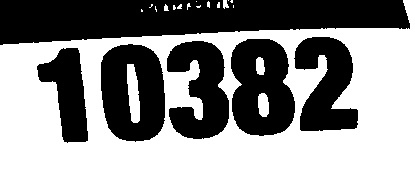
\includegraphics[width=\textwidth]{images/processing/ocr/10382_inv}
    \caption{Binarised}
  \end{subfigure}
  \\ \bigskip
  \hspace{\fill}
  \begin{subfigure}[b]{0.23\textwidth}
    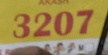
\includegraphics[width=\textwidth]{images/processing/ocr/3207_org}
    \caption{Original Image}
    \label{fig:processing_pipeline:ocr_postprocessing:color_original}
  \end{subfigure}
  \hspace{\fill}
  \begin{subfigure}[b]{0.23\textwidth}
    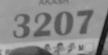
\includegraphics[width=\textwidth]{images/processing/ocr/3207_bw}
    \caption{Greyscale}
  \end{subfigure}
  \hspace{\fill}
  \begin{subfigure}[b]{0.23\textwidth}
    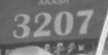
\includegraphics[width=\textwidth]{images/processing/ocr/3207_bw_inv}
    \caption{Inverse Greyscale}
  \end{subfigure}
  \hspace{\fill}
  
  \caption[Image post-processing applied to optimise input into an OCR engine]{Image post-processing applied to optimise input into an \gls{ocr} engine. \textit{Top}: An \gls{rbn} with white numbers can be applied binarised thresholding. \textit{Bottom}: A \gls{rbn} with red numbers cannot have binarised thresholding applied.}
  \label{fig:processing_pipeline:ocr_postprocessing}
\end{figure}

All preprocessed images are provided as input to Tesseract 4 alpha\footnoteurl{https://github.com/tesseract-ocr/tesseract/tree/4.00.00alpha}{5 September 2017}. We use this \gls{ocr} engine as it supports \gls{lstm} \gls{nn}-based character recognition. From all output of our various candidates shown in \cref{fig:processing_pipeline:ocr_postprocessing}, multiple text candidates are extracted from Tesseract. To clean our output, we strip out characters that are not within our known character range of A--Z, 0--9 and figure dashes. Additionally, we only accept unique \gls{rbn} sequences per bib region to prevent duplicates.
\section{Runtime Performance}

Our pipeline's runtime takes, on average, 23 seconds end-to-end per image (determined over all evaluations given in \cref{ch:evaluation}). \gls{ocr} and person detection runs in less than a second. The algorithmic complexity of our pipeline bottlenecks typically at the bib and text detection stages: when cropping is introduced in the pipeline, bib detection increases by a range of 2 to 10 extra seconds. Given the wide samples used to train the text detection network, this is the slowest stage, at an average of 13 seconds. Further breakdowns of the runtime performance is given in \cref{tab:results:summary:runtime}.

The engineering limitations of the \frcnn{} implementation may be improved architecturally by running the system at scale on a cloud cluster such as \gls{aws}. While memory complexity is not an issue, the time complexity is. We leave the improvements to our pipeline's runtime up to future works in systems architecture literature.

% Algorithm complexity...
% Person Detection, Bib Detection, Text Detection, Character Detection + OCR
% Discuss engineering limitations here of Keras FRCNN and talk about how we could improve it architecturally... time complexity just waft a bit about scale it up on AWS. Handball to architecture land/literature (future works). Memory complexity is also not an issue.

% Find paper that discusses OCR via NNs using Tesseract 4 alpha.
% Could discuss Luis's fallback pipeline?


\section{Summary}

This chapter presents an end-to-end pipeline that solely uses \glspl{nn} for object detection and text recognition to find the \glspl{rbn} in a given marathon photo. We successfully utilise transfer-learning on \frcnn{} to train it to detect both bibs sheets and text regions within those bib sheets. To reduce background noise, we use the \gls{yolo} object detection system and only check for bib sheets on a given crop of a detected human's bounding box region. We evaluate this pipeline in the following chapter.

\bigskip

\noindent
The primary contributions of this chapter are:

\begin{itemize}
  \item an end-to-end \gls{nn}-based pipeline to detect and recognise \glspl{rbn} in a natural scene, and
  \item a proposed method to increase accuracies by human extraction within photos.
\end{itemize}

\noindent
Minor contributions in this chapter include:

\begin{itemize}
  \item evolvement in the area of object detection and transfer learning,
  \item a methodology for improving the results from an \gls{ocr} system given images without binarised text colours, and
  \item a methodology for removing false positive cases from an \gls{ocr} system.
\end{itemize}